\scanpage{19}
\mspage{45}
en groupes \deleted{localement}\figure{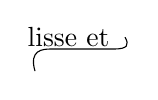
\begin{tikzpicture}[baseline=(a.base),x=1cm,y=1cm]
\node[anchor=west,inner sep=0pt] (a) at (0,0) {\inserted{lisse et}};
\draw ([xshift=.1cm,yshift=-.30cm]a.south west) .. controls ([xshift=.02cm,yshift=-.03cm]a.south west) and ([xshift=.2cm,yshift=-.02cm]a.south west) .. ([xshift=.3cm,yshift=-.02cm]a.south west) -- ([xshift=.05cm,yshift=-.02cm]a.south east) .. controls ([xshift=.22cm,yshift=-.02cm]a.south east) and ([xshift=.25cm,yshift=.03cm]a.south east) .. ([xshift=.19cm,yshift=.13cm]a.south east);
\end{tikzpicture}} de type fini sur $k$, soit $\uline{\operatorname{Pic}}_U$, et un isomorphisme
\[
\operatorname{Pic}(U)=\uline{\operatorname{Pic}}_U(k)
\tag{8.13}
\]
de $\operatorname{Pic}(U)$ avec le groupe des points à valeurs dans $k$ de $\uline{\operatorname{Pic}}_U$. Cela nous fournit donc pour $\operatorname{Pic}(U)$ une structure d'extension
\[
\diagram{\begin{tikzcd}[ampersand replacement=\&,column sep=small]
0\arrow[r]\&\operatorname{Pic}(U)^0\arrow[r]\&\operatorname{Pic}(U)\arrow[r]\&\operatorname{NS}(U)\arrow[r]\&0
\end{tikzcd}},
\tag{8.14}
\]
où on a posé
\[
\operatorname{Pic}(U)^0=\uline{\operatorname{Pic}}_U^0(k),\qquad\operatorname{NS}(U)=\uline{\operatorname{NS}}_U(k),
\tag{8.15}
\]
\deleted{\unsure{où}} $\uline{\operatorname{Pic}}_U^0$ désignant la composante neutre de $\uline{\operatorname{Pic}}_U$, et $\uline{\operatorname{NS}}_U$ le quotient de $\uline{\operatorname{Pic}}_U$ par cette composante. La construction indiquée dans loc. cit. permet d'ailleurs de préciser la structure de $\operatorname{NS}(U)$, en introduisant la matrice d'intersection
\[
(C_i.C_j)_{1\leq i,j\leq r}
\]
définie par les $r$ composantes irréductibles $C_i$ de $f^{-1}(x)_{\mathrm{r\acute ed}}$ sur le
\margin{\figure{\begin{tikzpicture}\draw (0,0)--(.18,.22);\draw (.03,.2)--(.16,.05);\end{tikzpicture}}}
schéma régulier $X'$ : en vertu de MUMFORD\figure{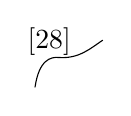
\begin{tikzpicture}[baseline=(b.base),x=1cm,y=1cm]
\node[anchor=west,inner sep=0pt] (b) at (0,0) {\inserted{[28]}};
\draw ([xshift=.10cm,yshift=-.40cm]b.south west) .. controls ([xshift=.15cm,yshift=-.05cm]b.south west) and ([xshift=.30cm,yshift=-.01cm]b.south west) .. ([xshift=.40cm,yshift=-.02cm]b.south west) .. controls ([xshift=.10cm,yshift=-.04cm]b.south east) and ([xshift=.25cm,yshift=.10cm]b.south east) .. ([xshift=.40cm,yshift=.20cm]b.south east);
\end{tikzpicture}}, cette matrice est définie négative, donc le conoyau de l'homomorphisme
\[
\uline{\mathrm Z}^{r}\longrightarrow\uline{\mathrm Z}^{r}
\]
qu'elle définit est un groupe fini, dont l'\unsure{ordre} n'est autre que la valeur absolue du déterminant de cette matrice. Ceci posé, on trouve que $\operatorname{NS}(U)$ est canoniquement isomorphe à ce groupe fini. La matrice envisagée étant symétrique, on voit aussitôt que ce groupe est canoniquement autodual (par un accouplement \deleted{\unsure{symétrique|canonique}}\inserted{\uline{symétrique}} à valeurs dans $\uline{\mathrm Q}/\uline{\mathrm Z}$), d'où une autodualité \figure{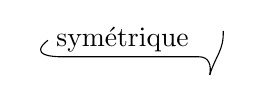
\begin{tikzpicture}[baseline=(c.base),x=1cm,y=1cm]
\node[anchor=west,inner sep=0pt] (c) at (0,0) {\inserted{symétrique}};
\draw ([xshift=-.10cm,yshift=.16cm]c.south west) .. controls ([xshift=-.35cm,yshift=-.04cm]c.south west) and ([xshift=-.03cm,yshift=-.05cm]c.south west) .. ([xshift=.08cm,yshift=-.05cm]c.south west) -- ([xshift=.12cm,yshift=-.05cm]c.south east) .. controls ([xshift=.25cm,yshift=-.05cm]c.south east) and ([xshift=.28cm,yshift=-.15cm]c.south east) .. ([xshift=.26cm,yshift=-.28cm]c.south east);
\draw ([xshift=.26cm,yshift=-.28cm]c.south east) .. controls ([xshift=.33cm,yshift=-.04cm]c.south east) and ([xshift=.44cm,yshift=.03cm]c.south east) .. ([xshift=.43cm,yshift=.28cm]c.south east);
\end{tikzpicture}}
\[
\operatorname{NS}(U)\times\operatorname{NS}(U)\longrightarrow\uline{\mathrm Q}/\uline{\mathrm Z},
\tag{8.16}
\]
dont on constate aisément qu'elle est indépendante de la résolution $X'$ choisie.

Si maintenant $\ell$ est un nombre premier distinct de $\operatorname{car}k$, alors la structure connue des groupes algébriques commutatifs connexes sur $k$ \inserted{[9, exp.4]} montre que $\operatorname{Pic}(U)_0$ est un groupe $\ell$-divisible, donc
\margin{\figure{\begin{tikzpicture}\draw (0,0)--(.18,.22);\draw (.03,.2)--(.16,.05);\end{tikzpicture}}}
\figure{\begin{tikzpicture}[x=.003cm,y=-.003cm]
\draw (535,170) .. controls (600,760) and (900,1600) .. (1100,2070);
\draw (270,840) .. controls (300,860) and (360,1600) .. (520,2080);
\draw (1235,60) .. controls (1310,270) and (1350,580) .. (1475,750);
\end{tikzpicture}}
\mspage{18}
